\chapter{Algorytmy}
\label{cha:algorytmy}

Istnieje wiele algorytmów do odkrywania struktury języka formalnego. Na przestrzeni lat powstało również wiele podejść i metod, które pomagają tworzyć zarówno rozwiązania ogólne, jak i te szczególnie efektywne w swojej niszy. Z uwagi na dużą liczbę dostępnych algorytmów zdecydowano się na ich ograniczony podzbiór, który wykorzystano w pracy. Są to \textit{L*}, \textit{RPNI}, \textit{GIG} i \textit{ALERGIA}, opisane kolejno w sekcjach \ref{sec:l-star}, \ref{sec:rpni}, \ref{sec:gig} i \ref{sec:alergia}. To właśnie te algorytmy przedstawiono jako pierwsze. Następnie krótko omówiono pozostałe algorytmy, które zostały uznane za interesujące, oraz wyjaśniono, dlaczego nie zdecydowano się na ich użycie.

\newenvironment{observationtable}[1][Tabela Obserwacji]{
  \begin{center}
  \renewcommand{\arraystretch}{1.3}
  \textbf{#1}\vspace{0.5em} \\
  \begin{tabular}{|c|c|c|}
  \hline
}{
  \hline
  \end{tabular}
  \end{center}
}

\section{Algorytm \textit{L*}}
\label{sec:l-star}

Algorytm \textit{L*} \cite{L_STAR} wyróżnia się na tle innych algorytmów do odkrywania gramatyki języka regularnego użytych w pracy dzięki swojemu podejściu do uczenia. Większość innych algorytmów opiera się wyłącznie na przykładach pozytywnych lub zarówno na przykładach pozytywnych, jak i negatywnych. Algorytm \textit{L*} wyłamuje się z tej konwencji, wykorzystując zapytania oraz kontrprzykłady do procesu nauki.

Model algorytmu składa się z dwóch aktorów: \textbf{nauczyciela} oraz \textbf{ucznia}. Jego celem jest skonstruowanie minimalnego deterministycznego automatu skończonego (DFA), który rozpoznaje dany język regularny na podstawie ograniczonych interakcji między dwoma uczestnikami procesu.

\subsection{Metoda}

Konstruowanie minimalnego automatu deterministycznego (DFA), który akceptuje język \( L \), odbywa się przy pomocy dwóch rodzajów zapytań:
\begin{enumerate}
    \item \textbf{Zapytania o członkostwo (Membership Queries, \textit{MQ}):} Uczeń pyta, czy słowo \( w \) należy do języka \( L \). Nauczyciel odpowiada „tak” (\( w \in L \)) lub „nie” (\( w \notin L \)).
    \item \textbf{Zapytania o równoważność (Equivalence Queries, \textit{EQ}):} Uczeń przedstawia hipotezę \( H \), reprezentującą język \( L(H) \), i pyta, czy \( L(H) = L \). Jeśli hipoteza jest niepoprawna, nauczyciel dostarcza kontrprzykład \( w \), dla którego \( w \in L \) i \( w \notin L(H) \), lub \( w \notin L \) i \( w \in L(H) \).
\end{enumerate}

Dla poprawnego działania algorytmu wymagane jest, aby nauczyciel mógł udzielać prawdziwych odpowiedzi na oba rodzaje zadawanych pytań. Nauczyciela często nazywa się również \textbf{wyrocznią}, co jest skrótem myślowym, ponieważ formalnie nauczyciel składa się z pary \textbf{wyroczni (oracles)}: \textit{MQ} i \textit{EQ}. Zazwyczaj to na użytkowniku algorytmu spoczywa odpowiedzialność za określenie nauczyciela, co wymaga już na wstępie posiadania pewnej wiedzy na temat danego języka. Jest to największe ograniczenie w zastosowaniu algorytmu \textit{L*}.

Proces algorytmu \textit{L*} opiera się na iteracyjnym konstruowaniu \textbf{tabeli obserwacji (Observation Table)}, która gromadzi informacje o języku L uzyskane na podstawie zapytań typu \textit{MQ}. Na podstawie zawartości tabeli formułowane są kolejne hipotezy dotyczące automatu DFA, które następnie poddawane są weryfikacji za pomocą zapytań typu \textit{EQ}.

Główne kroki algorytmu:
\begin{enumerate}
    \item \textbf{Inicjalizacja:} Algorytm rozpoczyna od utworzenia tabeli obserwacji wykorzystując minimalne zbiory prefiksów (\( S \)) i sufiksów (\( E \)).
    \item \textbf{Sprawdzanie domknięcia i spójności:} Algorytm weryfikuje, czy tabela obserwacji spełnia wymagania:
    \begin{itemize}
        \item \textbf{Domknięcie:} Każdy prefiks prowadzi do jednego z już znanych stanów.
        \item \textbf{Spójność:} Wiersze tabeli są rozróżnialne za pomocą sufiksów w \( E \).
    \end{itemize}
    Jeśli tabela nie spełnia tych wymagań algorytm zwiększa zbiory \( S \) i \( E \).
    \item \textbf{Tworzenie hipotezy:} Na podstawie tabeli obserwacji generowany jest automat DFA \( H \).
    \item \textbf{Test równoważności:} Hipoteza \( H \) jest testowana za pomocą \textit{EQ}. W przypadku błędu tabela jest aktualizowana na podstawie kontrprzykładu.
    \item \textbf{Terminacja:} Proces kończy się, gdy hipoteza \( H \) jest poprawna.
\end{enumerate}

\subsection{Formalizacja}

Celem tej sekcji jest przedstawienie formalnych podstaw i narzędzi matematycznych, które są niezbędne do zrozumienia algorytmu \( L^* \). W sekcji tej zawarto definicje kluczowych pojęć, takich jak języki regularne i automaty deterministyczne (DFA), które stanowią fundament problemu inferencji języka na podstawie ograniczonego zestawu danych.

\begin{definition}[DFA]
    \label{def:dfa}
    Skończony automat deterministyczny (DFA) to piątka uporządkowana
    \[ 
    M = (Q, \Sigma, \delta, q_0, F), 
    \]
    gdzie:
    \begin{itemize}
        \item \( Q \): skończony zbiór stanów,
        \item \( \Sigma \): alfabet,
        \item \( \delta: Q \times \Sigma \to Q \): funkcja przejścia,
        \item \( q_0 \in Q \): stan początkowy,
        \item \( F \subseteq Q \): zbiór stanów akceptujących.
    \end{itemize}
\end{definition}

\begin{definition}[Akceptowanie słowa]
    \label{def:word_acceptance}
    Automat \( M \) akceptuje słowo \( w \in \Sigma^* \), jeśli \( \delta(q_0, w) \in F \), gdzie \( \delta(q_0, w) \) oznacza iteracyjne zastosowanie funkcji przejścia \( \delta \) do słowa \( w \).
\end{definition}

\begin{definition}[Język regularny]  
    \label{def:regular_language}
    Język \( L \subseteq \Sigma^* \) zdefiniowany nad alfabetem \( \Sigma \) nazywamy językiem regularnym, jeśli istnieje deterministyczny automat skończony (DFA) \( M = (Q, \Sigma, \delta, q_0, F) \), który akceptuje wszystkie słowa należące do \( L \), i tylko te słowa:
    \[
    L = \{ w \in \Sigma^* \mid M \text{ akceptuje } w \}.
    \]
\end{definition}

Formalizacja DFA pozwala przejść od intuicyjnego opisu języka regularnego do jego precyzyjnej, algebraicznej reprezentacji. Stanowi to punkt wyjścia do rozważania procesu konstrukcji automatu \( H \) na podstawie tabeli obserwacji.

\begin{definition}[Tabela obserwacji] 
    Tabela obserwacji (ObservationTable) to struktura danych definiowana jako trójka \( (S, E, T) \), gdzie:
    \begin{itemize}
        \item \( S \subseteq \Sigma^* \): skończony zbiór prefiksów,
         \item \( E \subseteq \Sigma^* \): skończony zbiór sufiksów,
        \item \( T: (S \cup S \cdot \Sigma) \times E \to \{0, 1\} \): funkcja wartościująca wynik zapytania \( MQ(s \cdot e) \), gdzie \( s \in S \cup S \cdot \Sigma \) i \( e \in E \).
    \end{itemize}
\end{definition}

Tabela obserwacji jest kluczowym elementem algorytmu \( L^* \). Przechowuje informacje o zachowaniu języka \( L \) względem słów w zbiorach \( S \) i \( E \). Dzięki temu pozwala grupować słowa w klasy równoważności, co jest podstawą do wyznaczenia stanów DFA.

\begin{definition}[Domknięcie] 
    Tabela obserwacji jest domknięta jeśli dla każdego \( s \in S \cdot \Sigma \), istnieje \( s' \in S \), taki że \( \forall e \in E, \, T(s, e) = T(s', e) \).
\end{definition}
\begin{definition}[Spójność]
    Tabela obserwacji jest spójna, jeśli dla dowolnych \( s_1, s_2 \in S \), spełniających warunek:
    \[
    \forall e \in E, \, T(s_1, e) = T(s_2, e),
    \]
    zachodzi również:
    \[
    \forall a \in \Sigma, \, \forall e \in E, \, T(s_1 \cdot a, e) = T(s_2 \cdot a, e).
    \]
\end{definition}

Warunki te zapewniają, że tabela obserwacji reprezentuje wystarczająco bogatą informację o języku \( L \), aby można było skonstruować poprawny DFA. \textbf{Domknięcie} gwarantuje, że wszystkie przejścia są uwzględnione w zbiorze \( S \), natomiast \textbf{spójność} zapewnia, że tabela jest zgodna z oczekiwanym zachowaniem języka.

\begin{definition}[Tworzenie hipotezy]
    Na podstawie tabeli (ObservationTable), która spełnia warunki \textbf{domknięcia} i \textbf{spójności}, można skonstruować DFA \( H = (Q, \Sigma, \delta, q_0, F) \), gdzie:
    \begin{itemize}
        \item \( Q = \{[s] \mid s \in S\} \), gdzie \( [s] \) oznacza klasę równoważności \( s \) w \( T \),
        \item \( \delta([s], a) = [s \cdot a] \),
        \item \( q_0 = [\epsilon] \),
        \item \( F = \{[s] \mid T(s, \epsilon) = 1\} \).
    \end{itemize}
\end{definition}

Klasy równoważności w \( T \) grupują słowa \( s \in S \) o identycznym zachowaniu względem języka \( L \). Dzięki temu DFA \( H \) przechodzi między stanami odpowiadającymi tym klasom, w oparciu o funkcję przejścia \( \delta \).

\begin{definition}[Kontrprzykład]
    Kontrprzykład dla hipotezy H odnośnie języka L nazywamy takie $w$, że \( w \in L \setminus L(H) \cup L(H) \setminus L \).
\end{definition}

\begin{definition}[Zapytanie o członkostwo]
    \emph{Zapytanie o członkostwo} (\emph{Membership Query}) to funkcja \( MQ: \Sigma^* \to \{0, 1\} \), która dla danego słowa \( w \in \Sigma^* \) zwraca \( 1 \), jeśli \( w \in L \), lub \( 0 \) w przeciwnym przypadku.
\end{definition}

\begin{definition}[Zapytanie o równoważność]
    \emph{Zapytanie o równoważność} (\emph{Equivalence Query}) to funkcja \( EQ: \mathcal{H} \to (\Sigma^* \cup \{\text{brak}\}) \), która dla hipotezy \( H \) zwraca:
    \begin{itemize}
        \item brak, jeśli \( L(H) = L \), czyli hipoteza \( H \) jest równoważna językowi \( L \).
        \item w przeciwnym wypadku \textbf{kontrprzykład},
    \end{itemize}
\end{definition}


Jeśli język generowany z hipotezy \( H \) nie jest równoważny \( L \), Nauczyciel dostarcza kontrprzykład \( w \). Prefiksy \( w \) są dodawane do \( S \), a tabela jest aktualizowana zgodnie z wynikami zapytań \( MQ \). Proces ten jest iteracyjny i pozwala na sukcesywne udoskonalanie tabeli obserwacji oraz hipotezy automatu \( H \), aż do uzyskania poprawnego modelu języka.

% \subsection{Złożoność}

% Algorytm \textit{L*} składa się z kilku etapów, których złożoność można szczegółowo przeanalizować. Złożoność czasowa algorytmu jest wielomianowa, co zostało udowodnione \cite{L_STAR}. Aby wyliczyć złożoność pamięciową trzeba zdefiniować:
% \begin{itemize}
%     \item \(n\) - liczba stanów szukanego minimalnego DFA,
%     \item \(m\) - maksymalna długość kontrprzykładu,
%     \item \(|\Sigma|\) - rozmiar alfabetu.
% \end{itemize}

% Struktura danych w algorytmie składa się z dwóch komponentów:
% \begin{enumerate}
%     \item \textbf{Tabela obserwacji:}
%     \begin{itemize}
%         \item Zbiór \(S\) (prefiksy): maksymalnie \(O(n + m \cdot (n - 1))\) wpisów,
%         \item Zbiór \(E\) (sufiksy): maksymalnie \(O(n)\) wpisów,
%         \item Całkowity rozmiar tabeli: \(O(n \cdot m)\).
%     \end{itemize}
%     \item \textbf{DFA hipotezy:} DFA może mieć maksymalnie \(n\) stanów i \(O(n \cdot |\Sigma|)\) przejść.
% \end{enumerate}

% Algorytm wymaga pamięci na tabelę obserwacji oraz strukturę DFA, stąd można obliczyć łączną złożoność pamięciową:
% \[
% O(n \cdot m + n \cdot |\Sigma|).
% \]

% Podsumowując czynnikami wpływającymi na złożoność pamięciową są:
% \begin{itemize}
%     \item \textbf{Rozmiar alfabetu (\(|\Sigma|\))}: Większy alfabet oznacza więcej przejść w tabeli obserwacji i DFA.
%     \item \textbf{Długość kontrprzykładów (\(m\))}: Dłuższe kontrprzykłady zwiększają liczbę zapytań o członkostwo i rozmiar tabeli obserwacji.
%     \item \textbf{Liczba stanów DFA (\(n\))}: Więcej stanów oznacza większą tabelę obserwacji i więcej iteracji algorytmu.
% \end{itemize}

\subsection{Przykład działania}

Aby rozjaśnić działanie algorytmu \textit{L*}, rozważmy prosty język $L$:

\[
L = \{ w \in \{a, b\}^* \mid \text{liczba liter } a \text{ jest parzysta lub liczba liter } b \text{ jest parzysta} \}.
\]

DFA dla języka $L$ zawiera cztery stany, ponieważ istnieją cztery możliwe kombinacje parzystości:
\begin{enumerate}
    \item Stan $s_0$: parzysta liczba $a$ i parzysta liczba $b$,
    \item Stan $s_1$: nieparzysta liczba $a$ i parzysta liczba $b$,
    \item Stan $s_2$: nieparzysta liczba $a$ i nieparzysta liczba $b$,
    \item Stan $s_3$: parzysta liczba $a$ i nieparzysta liczba $b$.
\end{enumerate}

Schemat minimalnego DFA można zobaczyć na rysunku \ref{fig:dfa_even_a_or_even_b}.

\begin{figure}[ht]
    \centering
    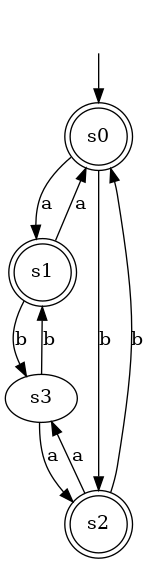
\includegraphics[width=0.2\linewidth]{images/dfa_even_a_or_even_b.png}
    \caption{Minimalny DFA dla języka $L$.}
    \label{fig:dfa_even_a_or_even_b}
\end{figure}

\paragraph*{Inicjalizacja tabeli obserwacji.}
Rozpoczynamy od tworzenia minimalnych zbiorów \textit{S} i \textit{E}:
\[
S = \{\epsilon\}, \quad E = \{\epsilon\}.
\]
Uczeń zadaje pytanie o członkostwo dla każdego elementu zbioru \( S \cup (S \cdot \Sigma) \):
\[
MQ(\epsilon) = 1, \quad MQ(a) = 1, \quad MQ(b) = 1.
\]
Wynik tego etapu można zobaczyć w tabeli \ref{tab:observation_1}. Jest ona \textbf{spójna} i \textbf{domknięta}. Można, więc skonstruować hipotezę.

\begin{table}
    \centering
    \begin{tabular}{c|c}
        \diagbox{\( S \cup (S \cdot \Sigma) \)}{$E$} & \( \epsilon \) \\
        \hline
        $\epsilon$      & 1 \\
        \hline
        $a$             & 1 \\
        $b$             & 1 \\
    \end{tabular}
    \caption{Początkowa tabela obserwacji.}
    \label{tab:observation_1}
\end{table}

\paragraph*{Konstrukcja hipotezy $H_1$.}
Na podstawie tabeli obserwacji \ref{tab:observation_1} konstruujemy hipotezę:
\begin{itemize}
    \item \textbf{Stany DFA:} \( q_\epsilon \), odpowiadający unikalnym wierszom tabeli.
    \item \textbf{Przejścia:}
    \begin{align*}
        & q_\epsilon \xrightarrow{a} q_\epsilon, \quad q_\epsilon \xrightarrow{b} q_\epsilon.
    \end{align*}
    \item \textbf{Stan początkowy:} \( q_\epsilon \).
    \item \textbf{Stany akceptujące:} \( q_\epsilon \).
\end{itemize}

\paragraph*{Testowanie hipotezy $H_1$.}
Hipoteza jest testowana przez zapytanie o równoważność ($EQ$). Można wybrać nieskończenie wiele kontrprzykładów, ale na potrzebę przykładu przyjmijmy, że nauczyciel zwraca $ba$.

\paragraph*{Aktualizacja tabeli obserwacji.}
Po otrzymaniu kontrprzykładu \( ba \), algorytm aktualizuje tabelę obserwacji. Wszystkie prefiksy \( ba \) są dodawane do zbioru \( S \), co prowadzi do:
\[
S = \{\epsilon, b, ba\}.
\]
Uczeń zadaje zapytania \( MQ \) dla nowych elementów \( S \cup (S \cdot \Sigma) \). Wyniki zapytań są następujące:
\[
MQ(ba) = 0, \quad MQ(baa) = 1, \quad MQ(bab) = 1.
\]
Wynikową tabelę obserwacji pokazano w tabeli \ref{tab:observation_2}. Jest ona \textbf{domknięta}, lecz \textbf{niespójna}, ponieważ:
\[
T(\epsilon, \epsilon) = T(b, \epsilon) \wedge T(\epsilon \cdot a, \epsilon) \neq T(b \cdot a, \epsilon),
\]
stąd $a$ jest rozróżniającym sufiksem. Dodajemy $a$ do $E$ i uzupełniamy tabelę obserwacji \ref{tab:observation_3}:
\[
MQ(\epsilon \cdot a) = 1, \quad MQ(b \cdot a) = 0, \quad MQ(ba \cdot a) = 1,
\]
\[
MQ(a \cdot a) = 1, \quad MQ(bb \cdot a) = 1, \quad MQ(baa \cdot a) = 0, \quad MQ(bab \cdot a) = 1.
\]
Tabela obserwacji jest teraz \textbf{domknięta} i \textbf{spójna}, więc możemy skonstruować hipotezę.

\begin{table}
    \centering
    \begin{tabular}{c|c}
        \diagbox{\( S \cup (S \cdot \Sigma) \)}{$E$} & \( \epsilon \) \\
        \hline
        $\epsilon$      & 1 \\
        $b$             & 1 \\
        $ba$            & 0 \\
        \hline
        $a$             & 1 \\
        $bb$            & 1 \\
        $baa$           & 1 \\
        $bab$           & 1 \\
    \end{tabular}
    \caption{Tabela obserwacji po otrzymaniu kontrprzykładu $ba$.}
    \label{tab:observation_2}
\end{table}

\begin{table}
    \centering
    \begin{tabular}{c|c|c}
        \diagbox{\( S \cup (S \cdot \Sigma) \)}{$E$} & \( \epsilon \) & $a$ \\
        \hline
        $\epsilon$      & 1 & 1 \\
        $b$             & 1 & 0 \\
        $ba$            & 0 & 1 \\
        \hline
        $a$             & 1 & 1 \\
        $bb$            & 1 & 1 \\
        $baa$           & 1 & 0 \\
        $bab$           & 1 & 1 \\
    \end{tabular}
    \caption{Tabela obserwacji po rozszerzeniu $E$ o element $a$.}
    \label{tab:observation_3}
\end{table}

\paragraph*{Konstrukcja hipotezy $H_2$.}
Na podstawie tabeli obserwacji \ref{tab:observation_3} konstruujemy hipotezę:
\begin{itemize}
    \item \textbf{Stany DFA:} \( q_\epsilon, q_b, q_{ba} \).
    \item \textbf{Przejścia:}
    \begin{align*}
        & q_\epsilon \xrightarrow{a} q_\epsilon, \quad q_\epsilon \xrightarrow{b} q_b, \\
        & q_b \xrightarrow{a} q_{ba}, \quad q_b \xrightarrow{b} q_\epsilon, \\
        & q_{ba} \xrightarrow{a} q_\epsilon, \quad q_{ba} \xrightarrow{b} q_b.
    \end{align*}
    \item \textbf{Stan początkowy:} \( q_\epsilon \).
    \item \textbf{Stany akceptujące:} \( q_\epsilon, q_b \).
\end{itemize}

\paragraph*{Testowanie hipotezy $H_2$.}
Hipoteza jest testowana przez zapytanie o równoważność ($EQ$). Ponownie można wybrać nieskończenie wiele kontrprzykładów. Przyjmijmy, więc, że nauczyciel zwraca $ab$.

\paragraph*{Aktualizacja tabeli obserwacji.}
Po otrzymaniu kontrprzykładu \( ab \), algorytm aktualizuje tabelę obserwacji. Na początek dodajemy \( a \) oraz \( ab \) do zbioru \( S \):
\[
S = \{ \epsilon, a, b, ab, ba \}.
\]
Uczeń zadaje pytania \( MQ \) dla nowych elementów zbioru \( S \cup (S \cdot \Sigma) \). Na tej podstawie aktualizujemy tabelę obserwacji. Wynikową tabelę obserwacji pokazano w tabeli \ref{tab:observation_4}. Tabela jest teraz \textbf{domknięta}, ale \textbf{niespójna}, ponieważ wiersz dla $\epsilon$ jest taki sam jak wiersz dla $a$, a wiersz dla \( \epsilon \cdot b \) jest inny niż wiersz dla \( a \cdot b \), stąd $b$ jest rozróżniającym sufiksem. Dodajemy $b$ do $E$ i uzupełniamy tabelę obserwacji \ref{tab:observation_5}. Dodanie \( b \) do \( E \) pozwala naprawić niespójność, rozróżniając zachowanie stanów dla różnych sufiksów.

\begin{table}
    \centering
    \begin{tabular}{c|c|c}
        \diagbox{\( S \cup (S \cdot \Sigma) \)}{$E$} & \( \epsilon \) & $a$ \\
        \hline
        $\epsilon$      & 1 & 1 \\
        $a$             & 1 & 1 \\
        $b$             & 1 & 0 \\
        $ab$            & 0 & 1 \\
        $ba$            & 0 & 1 \\
        \hline
        $aa$            & 1 & 1 \\
        $bb$            & 1 & 1 \\
        $aba$           & 1 & 0 \\
        $abb$           & 1 & 1 \\
        $baa$           & 1 & 0 \\
        $bab$           & 1 & 1 \\
    \end{tabular}
    \caption{Tabela obserwacji po dodaniu $a$ i $ab$ do $S$.}
    \label{tab:observation_4}
\end{table}

\begin{table}
    \centering
    \begin{tabular}{c|c|c|c}
        \diagbox{\( S \cup (S \cdot \Sigma) \)}{$E$} & $\epsilon$ & $a$ & $b$ \\
        \hline
        $\epsilon$      & 1 & 1 & 1 \\
        $a$             & 1 & 1 & 0 \\
        $b$             & 1 & 0 & 1 \\
        $ab$            & 0 & 1 & 1 \\
        $ba$            & 0 & 1 & 1 \\
        \hline
        $aa$            & 1 & 1 & 1 \\
        $bb$            & 1 & 1 & 1 \\
        $aba$           & 1 & 0 & 1 \\
        $abb$           & 1 & 1 & 0 \\
        $baa$           & 1 & 0 & 1 \\
        $bab$           & 1 & 1 & 0 \\
    \end{tabular}
    \caption{Tabela obserwacji po dodaniu $b$ do $E$.}
    \label{tab:observation_5}
\end{table}

\paragraph*{Konstrukcja hipotezy $H_3$.}
Na podstawie tabeli obserwacji konstruujemy hipotezę $H_3$:
\begin{itemize}
    \item \textbf{Stany DFA:} \( q_\epsilon, q_a, q_b, q_{ab} \), odpowiadające unikalnym wierszom tabeli.
    \item \textbf{Przejścia:}
    \begin{align*}
        & q_\epsilon \xrightarrow{a} q_a, \quad q_\epsilon \xrightarrow{b} q_b, \\
        & q_a \xrightarrow{a} q_\epsilon, \quad q_a \xrightarrow{b} q_{ab}, \\
        & q_b \xrightarrow{a} q_{ab}, \quad q_b \xrightarrow{b} q_\epsilon, \\
        & q_{ab} \xrightarrow{a} q_b, \quad q_{ab} \xrightarrow{b} q_a.
    \end{align*}
    \item \textbf{Stan początkowy:} \( q_\epsilon \).
    \item \textbf{Stany akceptujące:} \( q_\epsilon, q_a, q_b \), ponieważ odpowiadają sytuacjom, w których parzystość jednego z \( a \) lub \( b \) jest spełniona.
    \item \textbf{Stany nieakceptujące:} \( q_{ab} \), ponieważ odpowiada sytuacji, w której zarówno \( a \), jak i \( b \) mają nieparzystą liczbę wystąpień.
\end{itemize}

\paragraph*{Testowanie hipotezy $H_3$.}
Hipoteza jest testowana przez zapytanie o równoważność (EQ). Nauczyciel odpowiada ,,tak'', co kończy działanie algorytmu.

\paragraph*{Ostateczny automat.}
Automat DFA reprezentujący język \( L \) ma następującą macierz przejść:
\[
\begin{array}{c|c|c}
\text{Stan} & a & b \\
\hline
\rightarrow * q_\epsilon & q_a & q_b \\
* q_a & q_\epsilon & q_{ab} \\
* q_b & q_{ab} & q_\epsilon \\
q_{ab} & q_b & q_a \\
\end{array}
\]

\section{Algorytm \textit{RPNI}}
\label{sec:rpni}

\section{Algorytm \textit{GIG}}
\label{sec:gig}

Algorytm \textit{GIG} (\textit{Grammatical Inference by Genetic search}) \cite{GIG}, podobnie jak algorytm \textit{RPNI}, jest przeznaczony do indukcji gramatyk regularnych na podstawie przykładów pozytywnych \( S^+ \) i negatywnych \( S^- \). Oba algorytmy opierają się na iteracyjnym łączeniu stanów w celu skonstruowania deterministycznego automatu skończonego (DFA), który jak najlepiej opisuje dane. W przypadku \textit{RPNI} znaleziony DFA zawsze jest minimalny i akceptuje wszystkie słowa z \( S^+ \), odrzucając słowa z \( S^- \). Natomiast wynik algorytmu \textit{GIG} nie jest jednoznacznie określony.

W algorytmie \textit{GIG} przestrzeń możliwych rozwiązań jest reprezentowana jako podziały stanów maksymalnego automatu kanonicznego (MCA, ang. maximal canonical automaton) zbudowanego na podstawie zbioru \( S^+ \). Przeszukiwanie tej przestrzeni odbywa się przy użyciu algorytmu genetycznego, który iteracyjnie modyfikuje populację podziałów poprzez operacje takie jak krzyżowanie i mutacja. Funkcja dopasowania (\textit{fitness}) ocenia jakość każdego rozwiązania, preferując modele akceptujące jak najwięcej słów z \( S^+ \), odrzucające \( S^- \), a jednocześnie minimalizujące liczbę stanów. W efekcie uzyskane rozwiązanie może nie być optymalne ani w pełni poprawne.

W przeciwieństwie do deterministycznego podejścia algorytmu \textit{RPNI}, \textit{GIG} wykorzystuje mechanizmy ewolucyjne, co umożliwia efektywne przeszukiwanie dużych i złożonych przestrzeni rozwiązań. Jest to szczególnie istotne w przypadkach, gdy liczba stanów automatu lub rozmiar zbioru przykładów uczących znacząco rośnie.

W tej sekcji nie zostanie przedstawiony przykład działania, ponieważ jest to standardowy algorytm genetyczny. Zamiast tego, w podsekcji \ref{sec:gig-formalizacja} zostaną zaprezentowane przykłady operacji genetycznych, które pomogą zrozumieć działanie programu.

\subsection{Metoda}

GIG wykorzystuje algorytm genetyczny do indukcji deterministycznego automatu skończonego na podstawie przykładów pozytywnych i negatywnych. Kluczowym założeniem metody jest reprezentacja stanów maksymalnego automatu skończonego (MCA) jako podziału, który w procesie ewolucji jest optymalizowany pod kątem minimalizacji liczby stanów oraz zgodności z danymi wejściowymi.
\begin{enumerate}
    \item \textbf{Budowa automatu maksymalnego (MCA):}
        Na podstawie zbioru \( S^+ \) tworzony jest maksymalny automat skończony (MCA), w którym każdy stan odpowiada unikalnemu prefiksowi słów z \( S^+ \). MCA akceptuje dokładnie \( S^+ \), lecz nie jest minimalny.
    \item \textbf{Reprezentacja podziału stanów:}
        Stany MCA są reprezentowane jako podziały, gdzie każda grupa w podziale odpowiada jednemu stanowi w wynikowym DFA. Początkowa populacja składa się z losowych podziałów oraz rozwiązań opartych na strukturze MCA.
    \item \textbf{Ewolucja populacji:}
        Algorytm genetyczny iteracyjnie modyfikuje populację, stosując:
        \begin{itemize}
            \item \textbf{Krzyżowanie:} Łączenie dwóch podziałów w celu stworzenia nowych rozwiązań, przy zachowaniu strukturalnej zgodności podziałów.
            \item \textbf{Mutację:} Wprowadzanie losowych zmian w podziałach, aby eksplorować nowe obszary przestrzeni rozwiązań.
        \end{itemize}
    \item \textbf{Ocena dopasowania osobników (\textit{fitness}):}
        Każdy osobnik jest oceniany na podstawie skonstruowanego z niego DFA. Wartość dopasowania jest wyznaczana na podstawie liczby stanów DFA, zgodności z \( S^+ \) oraz zdolności do odrzucania \( S^- \). Preferowane są mniejsze automaty, które poprawnie klasyfikują dane.
    \item \textbf{Zakończenie:}
        Algorytm kończy działanie po osiągnięciu określonej liczby generacji lub spełnieniu kryterium stopu (np. brak poprawy w kolejnych iteracjach). Wynikowy podział definiuje DFA zgodny z \( S^+ \) i \( S^- \).
\end{enumerate}

\subsection{Różnice podejścia genetycznego i zachłannego}

Algorytm \textit{GIG} ma przewagę nad klasycznym algorytmem \textit{RPNI} w kontekście indukcji gramatyk regularnych, szczególnie w przypadku dużych i złożonych zestawów danych. Kluczową różnicą między oboma podejściami jest sposób przeszukiwania przestrzeni rozwiązań. \textit{RPNI} działa deterministycznie, łącząc stany automatu maksymalnego (PTA) w oparciu o reprezentatywność danych \( S^+ \) i \( S^- \), co pozwala na konstrukcję minimalnego automatu skończonego (DFA). Jednakże, w przypadku bardzo dużych przestrzeni rozwiązań algorytm deterministyczny może zawieść, nie będąc w stanie efektywnie eksplorować wszystkich możliwych podziałów.

W odróżnieniu od tego, \textit{GIG} wykorzystuje podejście ewolucyjne, co pozwala na bardziej elastyczne przeszukiwanie przestrzeni rozwiązań. Dzięki stochastycznemu charakterowi algorytmu genetycznego, \textit{GIG} jest w stanie znaleźć akceptowalne rozwiązanie, nawet jeśli nie jest ono optymalne. To podejście pozwala na radzenie sobie z ogromnymi zbiorami danych oraz sytuacjami, w których liczba stanów w automacie maksymalnym (MCA) znacząco wzrasta. Operacje genetyczne, takie jak krzyżowanie i mutacja, umożliwiają eksplorację przestrzeni podziałów w sposób mniej deterministyczny, zwiększając szansę na znalezienie rozwiązań w złożonych przypadkach.

Jednakże, w przeciwieństwie do deterministycznego podejścia \textit{RPNI}, algorytm \textit{GIG} nie gwarantuje, że uzyskane rozwiązanie będzie optymalne ani w pełni poprawne. Wynik może być jedynie przybliżeniem minimalnego automatu akceptującego \( S^+ \) i odrzucającego \( S^- \), co oznacza, że pewne nieścisłości w klasyfikacji mogą pozostać. Ponadto, czas działania \textit{GIG} jest uzależniony od parametrów takich jak liczba generacji i rozmiar populacji, co w niektórych przypadkach może prowadzić do wysokich kosztów obliczeniowych.

Dodatkowo, \textit{GIG} charakteryzuje się większą adaptacyjnością. Może dynamicznie dostosowywać populację oraz kryteria dopasowania (\textit{fitness}) do specyficznych cech problemu, co czyni go bardziej elastycznym w porównaniu do \textit{RPNI}. W sytuacjach, gdy przestrzeń stanów staje się zbyt duża dla deterministycznych podejść, \textit{GIG} potrafi efektywnie przeszukiwać tę przestrzeń dzięki heurystykom genetycznym, minimalizując ryzyko przeoczenia akceptowalnych rozwiązań.

Podsumowując, główną przewagą \textit{GIG} jest jego zdolność do radzenia sobie z ogromnymi zestawami danych oraz bardziej złożonymi strukturami języka, dzięki czemu może znaleźć rozwiązania, które są niedostępne dla deterministycznego podejścia \textit{RPNI}. Niemniej jednak, brak gwarancji optymalności i pełnej poprawności może być istotną wadą w sytuacjach wymagających precyzyjnych wyników.

\subsection{Formalizacja}
\label{sec:gig-formalizacja}

W tej sekcji opisano sposób przedstawienia rozwiązania w osobniku, proces inicjalizacji populacji, operatory genetyczne oraz funkcję przystosowania, która kieruje ewolucją. Dla każdego z tych elementów podano odpowiednie przykłady. Potrzebnymi definicjami dla tej sekcji będą definicja \ref{def:state_merging}, ponieważ łączenie stanów w \textit{GIG} przebiega w ten sam sposób co w \textit{RPNI}, oraz definicja \ref{def:pta}, jako że MCA w \textit{GIG} to dokładnie taka sama struktura co PTA w kontekście algorytmu \textit{RPNI}.

\paragraph*{Reprezentacja osobnika.}  
Każdy osobnik w populacji jest reprezentowany jako podział zbioru stanów \( Q \) automatu maksymalnego (MCA). Podział jest zakodowany jako wektor liczb całkowitych \( \mathbf{p} \), gdzie \( \mathbf{p}[i] = c \) oznacza, że stan \( q_i \in Q \) należy do grupy \( c \). Grupy odpowiadają stanom wynikowego deterministycznego automatu skończonego (DFA). Przykładowo, jeśli \( Q = \{q_0, q_1, q_2, q_3\} \), podział \( \mathbf{p} = [0, 0, 1, 1] \) oznacza, że stany \( q_0 \) i \( q_1 \) należą do jednej grupy, a \( q_2 \) i \( q_3 \) do drugiej.

Dla zapewnienia jednoznaczności i porównywalności osobników w populacji, podział \( \mathbf{p} \) musi być w formie kanonicznej. Oznacza to, że grupy w \( \mathbf{p} \) są ponumerowane w sposób ciągły, począwszy od \( 0 \), bez przeskoków w numeracji. Kanoniczność jest kluczowa, ponieważ pozwala unikać niejednoznaczności przy reprezentacji tego samego podziału oraz ułatwia operacje genetyczne, takie jak krzyżowanie i mutacja.

\textbf{Przykład:}  
Dla \( Q = \{q_0, q_1, q_2, q_3\} \), podział \( \mathbf{p} = [0, 2, 2, 5] \) nie jest kanoniczny, ponieważ grupy są ponumerowane z przeskokami (brakuje grup \( 1 \) i \( 3, 4 \)). Aby naprawić ten podział, każdej unikalnej wartości w \( \mathbf{p} \) przypisujemy nową numerację w kolejności ich występowania:
\[
\text{Niekanoniczny: } \mathbf{p} = [0, 2, 2, 5] \quad \rightarrow \quad \text{Kanoniczny: } \mathbf{p} = [0, 1, 1, 2].
\]

Naprawianie podziału jest procesem prostym, a dzięki kanonicznej formie reprezentacji różne osobniki o tej samej strukturze nie będą traktowane jako różne w trakcie ewolucji.

\paragraph*{Inicjalizacja populacji.}  
Początkowa populacja jest generowana w następujący sposób:
\begin{itemize}
    \item \textbf{Pierwszy osobnik:}  
    Pierwszy osobnik odpowiada obecnie rozszerzonemu automatowi (MCA), w którym każdy stan \( q_i \in Q \) należy do osobnej grupy. Przykładowo, dla \( Q = \{q_0, q_1, q_2, q_3\} \), pierwszy osobnik to \( \mathbf{p} = [0, 1, 2, 3] \).
    
    \item \textbf{Podziały z ograniczoną liczbą grup:}  
    Do 50\% populacji stanowią losowe podziały wybrane z \( \binom{|Q|}{2} \) możliwych podziałów, w których liczba grup wynosi \( |Q| - 1 \). Przykładowo, dla \( Q = \{q_0, q_1, q_2, q_3\} \), losowy podział może wyglądać tak: \( \mathbf{p} = [0, 0, 1, 2] \), gdzie \( q_0 \) i \( q_1 \) należą do tej samej grupy, a \( q_2 \) i \( q_3 \) są przypisane do osobnych grup.
    
    \item \textbf{Całkowicie losowe podziały:}  
    Pozostałe osobniki w populacji są generowane w sposób całkowicie losowy. Dla \( Q = \{q_0, q_1, q_2, q_3\} \), przykładowy losowy podział może wyglądać tak: \( \mathbf{p} = [0, 1, 1, 0] \), gdzie \( q_0 \) i \( q_3 \) należą do jednej grupy, a \( q_1 \) i \( q_2 \) do innej.
\end{itemize}

Takie podejście pozwala na inicjalizację populacji zarówno w oparciu o strukturalnie uzasadnione podziały, jak i bardziej eksploracyjne rozwiązania, zwiększając różnorodność przestrzeni początkowych rozwiązań.

\paragraph*{Mutacja.}  
Mutacja to operator genetyczny, który wprowadza losowe zmiany w reprezentacji osobnika \( \mathbf{p} \), pozwalając na eksplorację nowych podziałów przestrzeni rozwiązań. Formalnie, mutacja działa w następujący sposób:

Dla wybranego osobnika \( \mathbf{p} \), wybierany jest losowy indeks \( i \), gdzie 
\[ i \in \{0, 1, \dots, |Q|-1\}. \]

Wartość \( \mathbf{p}[i] \), odpowiadająca grupie przypisanej stanowi \( q_i \), jest zastępowana przez nową wartość \( c \), gdzie:
\[
c \in \{0, 1, \dots, \max(\mathbf{p}) + 1\}.
\]
Nowa wartość \( c \) może odpowiadać istniejącej grupie w \( \mathbf{p} \) lub utworzeniu nowej grupy. Po wykonaniu mutacji, wynikowy osobnik \( \mathbf{p}' \) jest kanonicznie porządkowany, aby zapewnić jednoznaczność reprezentacji.

\textbf{Przykład:}  
Dla osobnika \( \mathbf{p} = [0, 0, 1, 1] \), losowo wybrany indeks \( i = 3 \) (stan \( q_3 \)) prowadzi do zmiany wartości \( \mathbf{p}[3] \). Jeśli nowa wartość \( c \) to \( 2 \), to zmodyfikowany osobnik ma postać \( \mathbf{p}' = [0, 0, 1, 2] \). Po kanonicznej normalizacji osobnik pozostaje niezmieniony, ponieważ reprezentacja jest już poprawna.

\paragraph*{Krzyżowanie.}  
Krzyżowanie w algorytmie \textit{GIG} odbywa się w przestrzeni podziałów i polega na łączeniu wybranych bloków dwóch rodziców w celu utworzenia nowych osobników. Formalnie, dla dwóch rodziców \( \mathbf{p}_1 \) i \( \mathbf{p}_2 \), reprezentujących podziały \( \mathcal{P}_1 \) i \( \mathcal{P}_2 \), wybierane są losowe bloki \( B_1 \in \mathcal{P}_1 \) oraz \( B_2 \in \mathcal{P}_2 \). Bloki te są łączone w nowy blok \( B = B_1 \cup B_2 \), który zostaje wprowadzony do potomka. Nowy potomek dziedziczy pozostałe bloki od obojga rodziców, z uwzględnieniem połączenia. Po krzyżowaniu wynikowy podział jest normalizowany do postaci kanonicznej, aby zapewnić jednoznaczność reprezentacji osobnika.

\textbf{Przykład:}  
Dla dwóch rodziców:  
\[
\mathbf{p}_1 = [0, 0, 1, 1], \quad \mathbf{p}_2 = [0, 1, 1, 0],
\]
wybierane są bloki \( B_1 = \{q_0, q_1\} \) oraz \( B_2 = \{q_0, q_3\} \). Po połączeniu bloków \( B = B_1 \cup B_2 = \{q_0, q_1, q_3\} \), jeden z potomków może być reprezentowany jako:
\[
\mathbf{p} = [0, 0, 1, 0],
\]
gdzie \( q_0, q_1 \) i \( q_3 \) należą do jednej grupy, a \( q_2 \) do osobnej. Normalizacja potwierdza poprawność kanonicznej reprezentacji \( \mathbf{p} \).

\paragraph*{Funkcja przystosowania.}  
Funkcja przystosowania ocenia jakość osobników na podstawie poprawności ich podziału w kontekście danych \( S^+ \) i \( S^- \). Na przykład, DFA skonstruowany na podstawie osobnika \( \mathbf{p} = [0, 0, 1] \) może akceptować wszystkie słowa z \( S^+ \), ale odrzucać jedno słowo z \( S^- \), co obniża jego wartość przystosowania. Osobnik, który zarówno poprawnie akceptuje \( S^+ \), jak i odrzuca \( S^- \), uzyska wyższą wartość przystosowania.

\paragraph*{Proces ewolucji.}  
Algorytm iteracyjnie modyfikuje populację przez zastosowanie operatorów genetycznych (krzyżowanie i mutacja) oraz selekcję najlepszych osobników na podstawie funkcji przystosowania. Na przykład, w kolejnych generacjach populacja ewoluuje od początkowego rozwiązania \( \mathbf{p} = [0, 0, 1, 2] \) do \( \mathbf{p} = [0, 0, 0, 1] \), co prowadzi do uproszczonego automatu z mniejszą liczbą stanów.

\paragraph*{Wynik.}  
Rezultatem algorytmu jest DFA zminimalizowany na podstawie najlepszego osobnika końcowej populacji. Przykładowo, dla początkowego automatu MCA z czterema stanami \( Q = \{q_0, q_1, q_2, q_3\} \), wynikowy DFA może mieć tylko dwa stany, jeśli osobnik końcowy to \( \mathbf{p} = [0, 0, 1, 1] \).

\subsection{Złożoność}

W przypadku zastosowania algorytmu \textit{GIG} do indukcji gramatyk regularnych, złożoność czasowa zależy przede wszystkim od złożoności funkcji dopasowania i operatorów genetycznych, takich jak krzyżowanie i mutacja, które operują na podziałach stanów automatu maksymalnego (MCA). Liczba stanów \( Q \) w MCA oraz liczności zbiorów danych \( S^+ \) i \( S^- \) determinują koszt każdej generacji, ponieważ wpływają na czas potrzebny na konstrukcję automatu z danego podziału oraz sprawdzenie jego poprawności względem \( S^+ \) i \( S^- \).

W naszej konkretnej aplikacji nie mamy pewności, na ile wybrane operatory genetyczne oraz sposób kodowania problemu rzeczywiście oddają jego strukturę. Jest to kluczowa kwestia, ponieważ jakość dopasowania operatorów do problemu wpływa na tempo konwergencji algorytmu. Jeśli struktura problemu nie jest dobrze uchwycona przez funkcję dopasowania i operatory, algorytm może potrzebować więcej generacji, aby osiągnąć akceptowalne rozwiązanie. W praktyce nie jesteśmy w stanie przewidzieć, jak szybko algorytm będzie znajdował rozwiązania o wysokiej jakości, co sprawia, że jedynym sposobem na ocenę jego efektywności jest eksperymentalne testowanie dla różnych rozmiarów danych.

Zapotrzebowanie pamięciowe algorytmu wynika z przechowywania populacji, gdzie każdy osobnik jest reprezentowany jako podział zbioru \( Q \). Wymagana pamięć jest proporcjonalna do \( P \cdot |Q| \), gdzie \( P \) to liczba osobników w populacji. Dodatkowo, konieczne jest przechowywanie maksymalnego automatu skończonego (MCA), który wymaga \( O(|Q| \cdot |\Sigma|) \) pamięci, gdzie \( |\Sigma| \) to rozmiar alfabetu. Ponieważ automaty wynikowe są konstruowane dynamicznie podczas oceny funkcji dopasowania, a nie przechowywane dla każdego osobnika, pamięć nie jest dodatkowo obciążona przez pełne reprezentacje DFA.

Podsumowując, złożoność algorytmu \textit{GIG} w naszym przypadku jest determinowana głównie przez rozmiar zbiorów \( S^+ \), \( S^- \), liczbę stanów \( Q \), oraz zdolność operatorów genetycznych do odzwierciedlenia struktury problemu. Ze względu na brak pewności co do jakości tego dopasowania, ocena efektywności algorytmu wymaga praktycznych eksperymentów, które pozwolą lepiej zrozumieć jego zachowanie przy różnych rozmiarach danych.

\section{Algorytm \textit{ALERGIA}}  
\label{sec:alergia}  

Algorytm \textit{ALERGIA} \cite{ALERGIA} jest stosowany do indukcji stochastycznych gramatyk regularnych. W przeciwieństwie do \textit{RPNI} lub \textit{GIG}, które zakładają obecność zarówno przykładów pozytywnych, jak i negatywnych, \textit{ALERGIA} opiera się wyłącznie na zbiorze przykładów pozytywnych. Umożliwia to jego zastosowanie w sytuacjach, gdzie dostęp do przykładów negatywnych jest ograniczony lub niemożliwy.  

Algorytm ten konstruuje deterministyczny stochastyczny automat skończony (DSFA) na podstawie drzewa akceptacji prefiksów (PTA) utworzonego z dostępnych danych. Proces uogólniania polega na łączeniu stanów automatu, przy jednoczesnym zachowaniu zgodności ze statystycznym rozkładem prawdopodobieństwa przejść między stanami. Decyzje o scalaniu są podejmowane na podstawie testów statystycznych, które zapewniają, że wynikowy model zachowuje probabilistyczne własności danych wejściowych.  

Jedną z kluczowych cech algorytmu \textit{ALERGIA} jest jego zdolność do indukcji gramatyk stochastycznych, co czyni go szczególnie przydatnym w zastosowaniach wymagających modelowania niepewności lub probabilistycznych wzorców zachowań. Dzięki swojej efektywności obliczeniowej algorytm ten znajduje zastosowanie w zadaniach takich jak rozpoznawanie wzorców, analiza sekwencji biologicznych oraz modelowanie języka naturalnego.

Algorytm działa iteracyjnie, testując kompatybilność stanów i łącząc te, które są statystycznie zgodne. Proces kończy się, gdy żadne dalsze scalenie nie jest możliwe bez naruszenia kryteriów statystycznych. Dzięki temu wynikowy automat nie tylko reprezentuje język generowany przez dane treningowe, ale także umożliwia estymację prawdopodobieństwa generacji nowych ciągów.


\subsection{Metoda}  
Algorytm \textit{ALERGIA} pozwala na indukcję deterministycznego stochastycznego automatu skończonego (DSFA), który przybliża rozkład prawdopodobieństwa danych wejściowych. Proces ten obejmuje następujące kroki:  

\begin{enumerate}  
    \item \textbf{Budowa akceptora drzewa prefiksów (PTA):}  
        Zbiór przykładów pozytywnych jest używany do zbudowania deterministycznego automatu reprezentującego dokładnie wszystkie sekwencje w danych.  
    \item \textbf{Iteracyjne łączenie stanów:}  
        Algorytm analizuje pary stanów w PTA i testuje ich zgodność statystyczną. Łączenie stanów jest realizowane tylko wtedy, gdy nie narusza statystycznej zgodności z danymi.  
    \item \textbf{Sprawdzanie zgodności:}  
        Kompatybilność stanów jest oceniana za pomocą testu Hoeffding'a.  
    \item \textbf{Zakończenie:}  
        Algorytm kończy działanie, gdy żadne dalsze scalenie stanów nie jest możliwe bez naruszenia zgodności statystycznej. Ostateczny automat aproksymuje rozkład probabilistyczny danych wejściowych.  
\end{enumerate}


\subsection{Formalizacja}  
W tej sekcji przedstawiono matematyczne podstawy algorytmu \textit{ALERGIA} oraz definicje kluczowych pojęć, które umożliwiają precyzyjne opisanie jego działania. Algorytm ten wykorzystuje akceptor drzewa prefiksów (PTA) jako strukturę początkową z definicji \ref{def:pta}. Proces formalizacji skupia się na mechanizmach scalania stanów, które pozwalają na stopniowe upraszczanie automatu przy jednoczesnym zachowaniu zgodności z probabilistycznymi wzorcami danych wejściowych.  

\begin{definition}[DSFA]  
\label{def:dsfa}
Stochastyczny, skończony automat deterministyczny to piątka uporządkowana
\[ 
A = (Q, \Sigma, \delta, q_0, P), 
\]
gdzie:  
\begin{itemize}  
    \item \( Q \) – skończony zbiór stanów,  
    \item \( \Sigma \) – alfabet,  
    \item \( \delta : Q \times \Sigma \to Q \) – funkcja przejścia,  
    \item \( q_0 \in Q \) – stan początkowy,  
    \item \( P: Q \times \Sigma \to [0, 1] \) – funkcja prawdopodobieństwa przejść, spełniająca:  
    \[
    \sum_{a \in \Sigma} P(q, a) \leq 1, \quad \forall q \in Q, \quad a \in \Sigma.
    \]  
\end{itemize}
\end{definition}

Automat \( A \) generuje język stochastyczny, w którym każda sekwencja symboli z \( \Sigma \) jest akceptowana z określonym prawdopodobieństwem, wyznaczanym przez funkcję \( P \).

\begin{definition}[Test Hoeffding’a]  
\label{def:hoeffding_test}
Test Hoeffding’a w algorytmie ALERGIA jest wykorzystywany do porównania dwóch stanów \( q_1, q_2 \) poprzez wyznaczenie granicy tolerancji \( \epsilon \), która określa maksymalną dopuszczalną różnicę między ich rozkładami. Granica tolerancji \( \epsilon \) jest obliczana jako:  
\[
\epsilon = \sqrt{\frac{1}{2} \ln\left(\frac{2}{\alpha}\right)} \left( \frac{1}{\sqrt{n_1}} + \frac{1}{\sqrt{n_2}} \right),
\]
gdzie:  
\begin{itemize}  
    \item \( n_1, n_2 \) – liczba obserwacji w stanach \( q_1 \) i \( q_2 \),  
    \item \( \alpha \) – poziom ufności określający dopuszczalny margines błędu.  
\end{itemize}  
\end{definition}

Test Hoeffding’a to statystyczna metoda oceny zgodności dwóch rozkładów prawdopodobieństwa, bazująca na nierówności Hoeffding’a. W kontekście algorytmu \textit{ALERGIA} test ten służy do sprawdzania, czy różnice między obserwowanymi częstościami przejść w stanach automatu można uznać za przypadkowe, czy też są one statystycznie istotne. W algorytmie \textit{ALERGIA} test Hoeffding’a porównuje rozkłady przejść pomiędzy stanami automatu. Jeśli różnice są mniejsze niż wyznaczony próg tolerancji, stany są uznawane za zgodne statystycznie i mogą zostać scalone. 

\begin{definition}[Zgodność stanów]  
\label{def:alergia_state_compatibility}
Dwa stany \( q_1, q_2 \in Q \) są uznawane za zgodne (kompatybilne), jeżeli spełnione są dwa warunki:  
\begin{enumerate}
    \item Funkcja prawdopodobieństwa przejść \( P \) dla każdego symbolu \( a \in \Sigma \) spełnia:  
    \[
    |P(q_1, a) - P(q_2, a)| \leq \epsilon.
    \]  
    \item Prawdopodobieństwa terminacji \( P_F \) spełnia:
    \[
    |P_F(q_1) - P_F(q_2)| \leq \epsilon,
    \]  
    gdzie \( \epsilon \) jest granicą wyznaczoną przez test Hoeffding’a.
\end{enumerate}
\end{definition} 

\begin{definition}[Łączenie stanów w \textit{ALERGIA}]  
\label{def:alergia_state_merging}  
Łączenie dwóch stanów \( q_1, q_2 \in Q \) w stochastycznym, skończonym automacie deterministycznym (DSFA) \( A = (Q, \Sigma, \delta, q_0, P) \) polega na zintegrowaniu informacji o przejściach oraz rozkładach prawdopodobieństwa w jeden wspólny stan. Proces ten obejmuje następujące kroki:  

\begin{enumerate}  
    \item Wierzchołek reprezentujący stan \( q_2 \) zostaje przypisany jako poddrzewo do stanu \( q_1 \) poprzez modyfikację drzewa prefiksów.  
    \item Funkcja przejścia zostaje zaktualizowana:  
    \[
    \delta'(q, a) =
    \begin{cases}  
        \delta(q_1, a) & \text{jeśli } \delta(q, a) = q_2, \\  
        \delta(q, a) & \text{w przeciwnym przypadku.}  
    \end{cases}  
    \]  
    \item Przejścia oraz rozkłady prawdopodobieństwa dla symboli \( a \) są łączone poprzez uśrednienie wagowe:  
    \[
    P'(q, a) = \frac{n_1 \cdot P(q_1, a) + n_2 \cdot P(q_2, a)}{n_1 + n_2},
    \]  
    gdzie \( n_1 \) i \( n_2 \) oznaczają liczby obserwacji dla stanów \( q_1 \) i \( q_2 \).  
    \item Następnie wszystkie dzieci stanu \( q_2 \) zostają przeniesione do stanu \( q_1 \). Jeśli stan \( q_1 \) posiada już przejście dla danego symbolu, częstotliwości są sumowane. W przeciwnym przypadku tworzony jest nowy węzeł:  
    \[
    P'(q_1, a) = P(q_1, a) + P(q_2, a).
    \]  
    Proces ten jest kontynuowany rekurencyjnie dla wszystkich dzieci stanu \( q_2 \).  
\end{enumerate}  
\end{definition}  

Łączenie stanów jest przeprowadzane wyłącznie wtedy, gdy dwa stany oraz pary ich dzieci odpowiadające przejściom tych samych symboli spełniają kryteria zgodności określone w definicji \ref{def:alergia_state_compatibility}. Scalanie obejmuje także sumowanie obserwacji oraz prawdopodobieństw dla poddrzew, co zapewnia zachowanie struktury probabilistycznej danych wejściowych. Proces kończy się, gdy żadne dalsze połączenia nie spełniają warunków zgodności.  

% \subsection{Złożoność}  
% Algorytm \textit{ALERGIA} cechuje się złożonością wielomianową, zależną od rozmiaru danych wejściowych. W analizie złożoności czasowej i pamięciowej uwzględniamy następujące parametry:  
% \begin{itemize}  
%     \item \(|S^+|\) - liczba przykładów pozytywnych,  
%     \item \( l^+ \) - maksymalna długość ciągu w \( S^+ \),  
%     \item \(|Q|\) - liczba stanów w automacie,  
%     \item \(|\Sigma|\) - liczba symboli w alfabecie.  
% \end{itemize}  

% \paragraph*{Złożoność czasowa.}  
% Algorytm \textit{ALERGIA} składa się z dwóch głównych etapów: budowy drzewa prefiksowego oraz iteracyjnego scalania stanów.  

% \subparagraph*{Budowa drzewa prefiksowego (PTA).}  
% Pierwszy etap polega na utworzeniu drzewa prefiksowego (Prefix Tree Acceptor, PTA) na podstawie zbioru przykładów pozytywnych. Każde słowo jest dodawane do drzewa, a jego prefiksy są reprezentowane jako kolejne węzły. Proces ten wymaga analizy wszystkich przykładów oraz ich symboli, co prowadzi do złożoności:  
% \[
% O(|S^+| \cdot l^+).
% \]  

% \subparagraph*{Iteracyjne scalanie stanów.}  
% Drugi etap obejmuje iteracyjne porównywanie par stanów pod kątem zgodności, wykorzystując test Hoeffding’a. Każda para stanów jest sprawdzana pod względem zgodności prawdopodobieństw przejść i terminacji, a następnie wykonywane są rekurencyjne analizy następników. Sprawdzenie każdej pary stanów obejmuje:
% \begin{itemize}  
%     \item Porównanie prawdopodobieństw przejść dla wszystkich symboli w alfabecie \( \Sigma \).  
%     \item Rekurencyjne sprawdzenie zgodności następników.  
%     \item Ewentualne scalanie stanów, co wiąże się z aktualizacją przejść i prawdopodobieństw.  
% \end{itemize}  

% Złożoność iteracyjnego scalania stanów wynosi:  
% \[
% O(|Q|^4 \cdot |\Sigma|).
% \]  

% \subparagraph*{Złożoność rzeczywista.}  
% W praktyce rzeczywista złożoność algorytmu jest często znacznie niższa niż teoretyczna granica. Wynika to z dwóch głównych czynników:  
% \begin{enumerate}
%     \item Algorytm wcześnie scala zgodne stany, zmniejszając liczbę analizowanych stanów w kolejnych iteracjach.  
%     \item Stany znajdujące się na końcu porządku przetwarzania (liście drzewa) mają niewielu następców lub w ogóle ich nie posiadają, co ogranicza liczbę rekurencyjnych wywołań.  
% \end{enumerate}  

% Z tego powodu empiryczna złożoność algorytmu jest często bliższa:  
% \[
% O(|Q|^3 \cdot |\Sigma|).
% \]  

% \paragraph*{Łączna złożoność.}  
% Podsumowując, całkowita złożoność czasowa algorytmu obejmuje budowę drzewa oraz iteracyjne porównania i scalania stanów:  
% \[
% O(|S^+| \cdot l^+ + |Q|^4 \cdot |\Sigma|).
% \]

% \paragraph*{Zależność liczby stanów \( Q \).}  
% Liczba stanów \( |Q| \) w automacie jest bezpośrednio zależna od danych wejściowych. W najgorszym przypadku każde słowo o długości \( l^+ \) wnosi dokładnie \( l^+ \) nowych stanów. Przy \( |S^+| \) przykładach liczba stanów może wynosić:  
% \[
% |Q| \leq |S^+| \cdot l^+.
% \]  
% Z tego powodu rzeczywista złożoność algorytmu jest silnie powiązana z rozmiarem zbioru przykładów i długością słów.   
% \[
% O((|S^+| \cdot l^+)^4 \cdot |\Sigma|).
% \]


% \paragraph*{Złożoność pamięciowa}  
% Algorytm przechowuje następujące struktury:  
% \begin{itemize}  
%     \item \textbf{Drzewo prefiksowe (PTA):}  
%     PTA składa się z \( O(|S^+| \cdot l^+) \) stanów, z których każdy może mieć do \( |\Sigma| \) przejść. Wymagana przestrzeń pamięci wynosi:  
%     \[
%     O(|S^+| \cdot l^+ \cdot |\Sigma|).
%     \]  

%     \item \textbf{Statystyki przejść:}  
%     Dla każdego stanu przechowywane są rozkłady prawdopodobieństw oraz dane statystyczne, co daje dodatkowy koszt pamięciowy:  
%     \[
%     O(|S^+| \cdot l^+).
%     \]  
% \end{itemize}  

% Łączna złożoność pamięciowa wynosi:  
% \[
% O(|S^+| \cdot l^+ \cdot |\Sigma|).
% \]  

% \paragraph*{Czynniki wpływające na złożoność}  
% Efektywność algorytmu \textit{ALERGIA} zależy przede wszystkim od liczby przykładów pozytywnych (\( S^+ \)) oraz długości słów (\( l^+ \)), które determinują rozmiar drzewa prefiksowego i liczbę stanów do analizy. Dodatkowo, większy alfabet (\( |\Sigma| \)) zwiększa liczbę możliwych przejść, co wpływa zarówno na czas obliczeń, jak i wymagania pamięciowe.

\subsection{Przykład działania}  
Aby zilustrować działanie algorytmu \textit{ALERGIA}, rozważmy prosty przykład danych wejściowych opisujących sekwencje wyników rzutów monetą. Każdy wynik jest oznaczony symbolem \( H \) (orzeł) lub \( T \) (reszka).

\paragraph*{Dane wejściowe.}  
Zbiór przykładów pozytywnych (\( S^+ \)):  
\[
S^+ = \{H, H, T, HH, HT, TH, TT, HHH\}.
\]  

\paragraph*{Krok 1: Konstrukcja drzewa prefiksowego (PTA).}  
Na podstawie danych pozytywnych algorytm buduje drzewo prefiksowe (Prefix Tree Acceptor, PTA), które reprezentuje dokładnie wszystkie obserwowane sekwencje. Każdy stan odpowiada prefiksowi słów z \( S^+ \), a przejścia są etykietowane symbolami \( H \) lub \( T \). Wynik tego kroku można zobaczyć na rysunku \ref{fig:alergia_example_0}. 

\begin{figure}[ht]
    \centering
    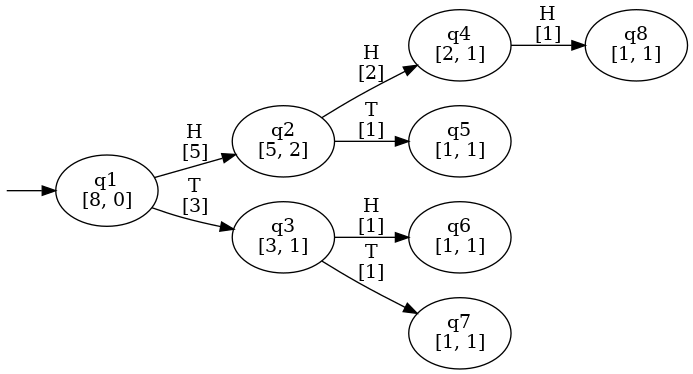
\includegraphics[width=0.8\textwidth]{images/run_example/alergia/0.png}
    \caption{Drzewo prefiksowe (PTA) skonstruowane dla \( S^+ \).}
    \label{fig:alergia_example_0}
\end{figure}

\paragraph*{Krok 2: Próba scalania stanów \( q_1 \) i \( q_2 \).}  
Algorytm rozpoczyna proces od analizy zgodności pierwszej pary stanów \( q_1 \) i \( q_2 \). Weryfikacja odbywa się na podstawie rozkładów prawdopodobieństw przejść oraz prawdopodobieństwa terminacji w obu stanach.  

\paragraph*{Dane stanów:}  
\begin{itemize}  
    \item \( q_1 \): \( n = 8, F = 0 \), przejścia: \( H[5], T[3] \).  
    \item \( q_2 \): \( n = 5, F = 2 \), przejścia: \( H[2], T[1] \).  
\end{itemize}  

\paragraph*{Sprawdzenie terminacji:}  
Prawdopodobieństwo terminacji dla każdego stanu:  
\[
P_F(q_1) = \frac{0}{8} = 0, \quad P_F(q_2) = \frac{2}{5} = \num{0.4},
\]

Różnica:  
\[
|P_F(q_1) - P_F(q_2)| = |0 - \num{0.4}| = \num{0.4}.
\]

\paragraph*{Tolerancja Hoeffding’a:}  
Przy poziomie ufności \( \alpha = \num{1.7} \) oraz liczbach obserwacji \( n_1 = 8 \) i \( n_2 = 5 \), granica zgodności \( \epsilon \) jest obliczana na podstawie wzoru:  
\[
\epsilon = \sqrt{\frac{\ln(2 / \alpha)}{2}} \left( \frac{1}{\sqrt{n_1}} + \frac{1}{\sqrt{n_2}} \right)
\]
\[
\epsilon \approx \num{0.228}.
\]

\paragraph*{Porównanie:}  
Ponieważ \( \num{0.4} > \num{0.228} \), stany \( q_1 \) i \( q_2 \) \textbf{nie mogą zostać połączone}.

\paragraph*{}

\paragraph*{Krok 3: Scalanie stanów \( q_2 \) i \( q_3 \).}  
Po odrzuceniu scalania stanów \( q_1 \) i \( q_2 \), algorytm przechodzi do analizy zgodności pary stanów \( q_2 \) i \( q_3 \).

\paragraph*{Dane stanów:}  
\begin{itemize}  
    \item \( q_2 \): \( n = 5, F = 2 \), przejścia: \( H[2], T[1] \), 
    \item \( q_3 \): \( n = 3, F = 1 \), przejścia: \( H[1], T[1] \).  
\end{itemize}  

\paragraph*{Test Hoeffding’a:}  
Prawdopodobieństwo terminacji dla każdego stanu:  
\[
P(q_2, H) = \frac{2}{5} = \num{0.4}, \quad P(q_3, H) = \frac{1}{3} \approx \num{0.333},
\]
\[
P(q_2, T) = \frac{1}{5} = \num{0.2}, \quad P(q_3, T) = \frac{1}{3} \approx \num{0.333},
\]
\[
P_F(q_2) = \frac{2}{5} = \num{0.4}, \quad P_F(q_3) = \frac{1}{3} \approx \num{0.333}.
\]

Różnica:  
\[
|P(q_2, H) - P(q_3, H)| \approx |\num{0.4} - \num{0.333}| = \num{0.067},
\]
\[
|P(q_2, T) - P(q_3, T)| \approx |\num{0.2} - \num{0.333}| = \num{0.133},
\]
\[
|P_F(q_2) - P_F(q_3)| \approx |\num{0.4} - \num{0.333}| = \num{0.067}.
\]

\paragraph*{Tolerancja Hoeffding’a:}  
Przy poziomie ufności \( \alpha = \num{1.7} \) oraz liczbach obserwacji \( n_1 = 5 \) i \( n_2 = 3 \), granica zgodności \( \epsilon \) jest obliczana na podstawie wzoru:  
\[
\epsilon = \sqrt{\frac{\ln(2 / \alpha)}{2}} \left( \frac{1}{\sqrt{n_1}} + \frac{1}{\sqrt{n_2}} \right)
\]
\[
\epsilon \approx \num{0.318}.
\]

\paragraph*{Porównanie:}  
Ponieważ:  
\[
|P(q_2, H) - P(q_3, H)| < \num{0.318}, \quad
\]
\[
|P(q_2, T) - P(q_3, T)| < \num{0.318}, \quad
\]
\[
|P_F(q_2) - P_F(q_3)| < \num{0.318},
\]  
stany \( q_2 \) i \( q_3 \) \textbf{są zgodne}. Aby mogły zostać połączone musimy sprawdzić rekurencyjnie zgodność dzieci stanu $q_3$ z odpowiednikami z gałęzi $q_2$, tj. $q_4$ i $q_6$ oraz $q_5$ i $q_7$. Analogiczne obliczenia wykazują zgodność wszystkich tych par stanów. Wynik tego kroku przedstawiono na rysunku \ref{fig:alergia_example_1}.  

\begin{figure}[ht]
    \centering
    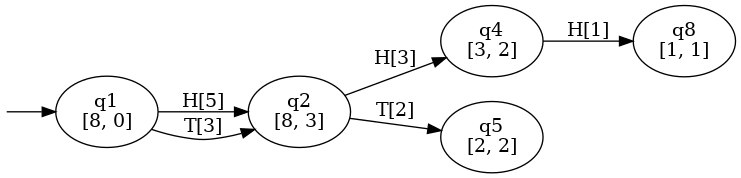
\includegraphics[width=0.8\textwidth]{images/run_example/alergia/1.png}
    \caption{Graf po scaleniu stanów \( q_2 \) i \( q_3 \).}
    \label{fig:alergia_example_1}
\end{figure}

\paragraph*{Krok 4: Scalanie stanów \( q_4 \) i \( q_8 \).}  
Po wcześniejszym scaleniu stanów \( q_2 \) i \( q_3 \), \( q_4 \) i \( q_6 \) oraz \( q_5 \) i \( q_7 \), algorytm przechodzi do następnej zgodnej pary stanów \( q_4 \) i \( q_8 \). Stan \( q_4 \) po wcześniejszym scaleniu z \( q_6 \) posiada \( n = 3, F = 2 \) oraz przejście \( H[1] \). Stan \( q_8 \) ma \( n = 1, F = 1 \) i brak przejść. Obliczenia są przeprowadzane analogicznie do wcześniejszych kroków. Porównanie prawdopodobieństw przejść oraz terminacji pokazuje, że różnice mieszczą się w zakresie tolerancji Hoeffding’a. Dzięki temu stany mogą zostać połączone, tworząc nowy stan \( q_4 \) o wartościach \( n = 4, F = 3 \) oraz przejściem zwrotnym \( H[1] \). Wynik tego kroku przedstawiono na rysunku \ref{fig:alergia_example_2}.  

\begin{figure}[ht]
    \centering
    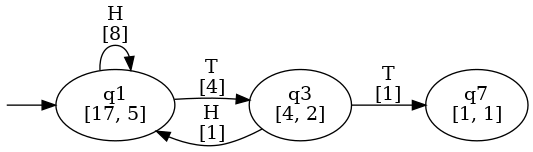
\includegraphics[width=0.8\textwidth]{images/run_example/alergia/2.png}
    \caption{Graf po scaleniu stanów \( q_4 \) i \( q_8 \).}
    \label{fig:alergia_example_2}
\end{figure}  

\paragraph*{Krok 5: Scalanie stanów \( q_4 \) i \( q_5 \).}  
Po wcześniejszych krokach, w których scalono stany \( q_2 \) z \( q_3 \), \( q_4 \) z \( q_6 \) oraz \( q_5 \) z \( q_7 \), algorytm przechodzi do analizy zgodności pary stanów \( q_4 \) i \( q_5 \). Stan \( q_4 \) po wcześniejszych operacjach posiada \( n = 3, F = 2 \) z przejściem zwrotnym \( H[1] \), natomiast stan \( q_5 \) ma \( n = 2, F = 2 \) i brak przejść. Obliczenia Hoeffding’a przeprowadzone w sposób analogiczny do wcześniejszych kroków pokazują, że różnice w rozkładach prawdopodobieństw przejść oraz terminacji mieszczą się w zakresie tolerancji. Dzięki temu stany zostają połączone, tworząc nowy stan \( q_4 \) z wartościami \( n = 5, F = 4 \) oraz przejściem zwrotnym \( H[1] \). Wynikowy graf można zobaczyć na rysunku \ref{fig:alergia_example_3}.

\begin{figure}[ht]
    \centering
    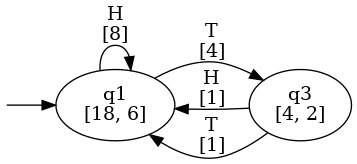
\includegraphics[width=0.8\textwidth]{images/run_example/alergia/3.png}
    \caption{Graf po scaleniu stanów \( q_4 \) i \( q_5 \).}
    \label{fig:alergia_example_3}
\end{figure}  

\paragraph*{Przekształcenie do postaci probabilistycznej.}  
W ostatnim kroku przekształcamy graf do postaci probabilistycznej. Prawdopodobieństwa terminacji oraz przejść są obliczane w sposób analogiczny do poprzednich kroków, uwzględniając wartości dla każdego stanu oraz przejść między nimi. Finalna postać grafu probabilistycznego reprezentuje rozkład danych wejściowych i umożliwia estymację nowych sekwencji. Wynikowy automat stochastyczny odwzorowuje prawdopodobieństwa przejść oraz terminacji, zapewniając zgodność probabilistyczną z danymi treningowymi. Wyniki tych kroków przedstawiono na rysunkach \ref{fig:alergia_example_4}.  

\begin{figure}[ht]
    \centering
    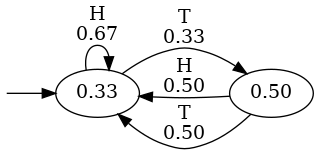
\includegraphics[width=0.8\textwidth]{images/run_example/alergia/4.png}
    \caption{Graf z probabilistycznymi przejściami i terminacjami.}
    \label{fig:alergia_example_4}
\end{figure}  

\paragraph*{Podsumowanie:}  
Algorytm zakończył proces scalania, redukując liczbę stanów i upraszczając strukturę automatu. Wynikowy automat stochastyczny zachowuje zgodność probabilistyczną z danymi wejściowymi, reprezentując ich rozkłady prawdopodobieństwa w sposób bardziej uogólniony. Finalna postać automatu pozwala na estymację nowych sekwencji zgodnych z rozkładem danych treningowych.  

